\newpage
\todo[inline]{General, use pont instead of comma for numerical values}
\section{Team Evaluation}
\label{sec:04_teamEvaluation}

\todo[inline]{It took me a while to understand that you evaluate the team-performance
with all TDOA methods here. The introduction should point that out so that the reader
is not surprised. (see my comment on "why did you choose GCC)}

In the preceding sections of this chapter the performance of the three
\ac{TDOA} methods were evaluated with respect to the prediction accuracy on
individual robots.
The remaining part of this chapter focuses on the performance of the joint
whistle localization using measurements of multiple agents. \todo{Find
a consistent term to talk about "joint whistle localization"}
Input to the joint whistle localization are the direction estimates of each
robot in the team. Base on these results, the team whistle localization outputs
an absolute sound source position. To provide a decoupled result to the signal
start detection, the start indexes were set manually. \todo{for the entire chapter?}
\todo[inline]{(outdated, see comment at the beginning of this section) Which
TDOA method did you end up using here and why? Maybe there needs to be }

% It is looked at the result of one exemplary measurement where the behavior
% of the team filter is of prime importance.


\subsection{GCC Method}
\label{04_teamGcc}

To determine an overall result, each robot computes a direction prediction from
the locally recorded signal using the \ac{GCC-PHAT} method standing
alone.\todo{I feel like the conclusion of "what is the best TDOA method" needs
to be before this section. Otherwise it is not clear why you use GCC-PHAT here}
These local direction estimates of individual robots are fed to the team
decision filter as specified in \cref{sec:03_teamDecision} which estimates the
global sound source position by combining all measurements through Bayesian
updates.

For further clarification, measurement 1 of \cref{subsec:04_labMeasurements} is
presented in greater detail as an example.
\Cref{fig:04_gccResult} illustrates the result of the relative direction
estimates $\gamma$ of the individual robots listed in \cref{tab:04_gccResult}
for this example.\todo{Maybe gamma should have a lower index}
For \cref{fig:04_setup,fig:04_gccResult}, robot positions are marked by yellow dots
where a short yellow line indicates each robot's orientation.
The arrows in \cref{fig:04_gccResult} represent the local direction estimates
$\gamma$ as predicted by each robot. Finally, the true position of the sound
source is marked with a red star while the joint position estimate over all
robots is visualized by a cross.
% -------------------------------------------------------------
\btline{ht}{1.2}
\btab{|c|c|c|c|}
\hline
NAO & $\gamma$ [\si{\deg}] & Abs. Error [\si{\deg}] & Mean PSNR \\
\hline
21 & -26.22 & 3.71 & 18.3\\
\hline
24 & -133.77 & 9.32 & 16.8\\
\hline
26 & -30.19 & 3.50 & 19.6\\
\hline
27 & -75.26 & 1.71 & 17.4\\
\hline
28 & -15.90 & 2.53 & 15.1\\
\hline
\etab
\et{Resulting direction estimates of the individual robots with \ac{GCC-PHAT}
method for a whistle sound signal in the right front corner of the playing
field}{04_gccResult} \todo[inline]{Does Abs Error refer to the true error or
the estimated error (e.g. uncertainty).}
% -------------------------------------------------------------
\begin{figure}[ht]
	\centering
		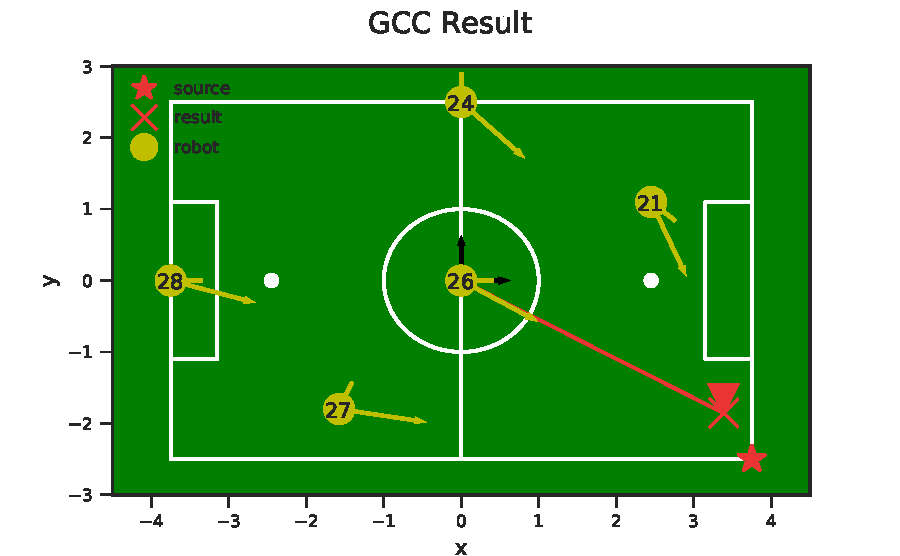
\includegraphics[]{figures/evaluation/gcc_team}
	\caption{Team whistle localization result with \ac{GCC-PHAT}
	method.}
    \label{fig:04_gccResult}
\end{figure}
% -------------------------------------------------------------

The final result and its corresponding errors are listed in
\cref{tab:04_gccTeamResult}. With an absolute distance error of less than
1\si{\meter} and small angular error, the source localization works
sufficiently for this case of application.
% -------------------------------------------------------------
\btline{ht}{1.2}
\btab{|c|c|c|}
\hline
 & Result & Error\\
\hline
Position x [\si{\meter}] & 3.38 & -0.37\\
\hline
Position y [\si{\meter}] & -1.85 & 0.65\\
\hline
Angle & 33.18\si{\degree} & 1.57\si{\degree}\\
\hline
Distance [\si{\meter}] & 3.85 & 0.74 \\
\hline
\etab
\et{Whistle localization result of measurement 1 with \ac{GCC-PHAT} method}{04_gccTeamResult}
% -------------------------------------------------------------

\Cref{tab:04_gccTeamResult} shows the distance and angle errors
for all measurements in \cref{subsec:04_labMeasurements}.
The \ac{RMSE} in distance being 0.87\si{\meter} and angular \ac{RMSE}
being 5.07\si{\degree} one can say that the \ac{GCC-PHAT} algorithm
works well for whistle sound source localization.
% -------------------------------------------------------------
\btline{ht}{1.2}
\btab{|c|c|c|c|c|}
\hline
Measurement & Error x [\si{\meter}] & Error y [\si{\meter}] & Abs. Distance Error [\si{\meter}] & Angle Error\\
\hline
0 & 1.31 & 1.06 & 1.68 & 1.45\si{\degree}\\
\hline
1 & 0.13 & 0.06 & 0.15 & 1.57\si{\degree}\\
\hline
2 & 0.59 & 0.43 & 0.73 & 0.42\si{\degree}\\
\hline
3 & 0.54 & 0.47 & 0.72 & 9.09\si{\degree}\\
\hline
4 & 0.27 & 0.0 & 0.27 & 0.01\si{\degree}\\
\hline
5 & 0.15 & 0.14 & 0.21 & 3.18\si{\degree}\\
\hline
6 & 0.41 & -0.02 & 0.41 & 2.67\si{\degree}\\
\hline
7 & 0.39 & 0.02 & 0.39 & 8.98\si{\degree}\\
\hline
8 & 1.84 & -0.01 & 1.84 & 0.14\si{\degree}\\
\hline
9 & 0.58 & 0.52 & 0.78 & 9.89\si{\degree}\\
\hline
10 & 0.03 & -0.0 & 0.03 & 0.0\si{\degree}\\
\hline
\etab
\et{Whistle localization results for all measurements in \cref{subsec:04_labMeasurements} with
\ac{GCC-PHAT} method}{04_gccTeamResult}
% -------------------------------------------------------------
% - intersections
% - updates
% - covariance
% - PSNR

% -------------------------------------------------------------
\subsection{CC Method}
\label{04_teamCc}

The \ac{CC} method is evaluated on the same data as in
\cref{subsec:04_labMeasurements}.\todo{You should probably just say this once
in the beginning (e.g. all evaluations use the same dataset).}
The results for the predictions of this method are reported in
\cref{tab:04_ccTeamResult}. Over all measurements, the \ac{CC} predictor has
a \ac{RMSE} of 1.45\si{\meter} in distance and 10.67\si{\degree} angular. The
results show that the standard \ac{CC} performs worse as compared to the
\ac{GCC-PHAT} method. Indeed, the statements in \cref{sec:02_cc} prove to be
true.

% -------------------------------------------------------------
\btline{ht}{1.2}
\btab{|c|c|c|c|c|}
\hline
Measurement & Error x [\si{\meter}] & Error y [\si{\meter}] & Abs. Distance Error [\si{\meter}] & Angle Error\\
\hline
0 & 0.6 & 1.39 & 1.51 & 8.15\si{\degree}\\
\hline
1 & -0.49 & 1.2 & 1.3 & 11.97\si{\degree}\\
\hline
2 & 2.32 & 2.11 & 3.13 & 18.28\si{\degree}\\
\hline
3 & 1.07 & -0.96 & 1.44 & 3.71\si{\degree}\\
\hline
4 & 1.95 & -0.09 & 1.95 & 10.44\si{\degree}\\
\hline
5 & 0.07 & 0.01 & 0.07 & 0.32\si{\degree}\\
\hline
6 & 0.4 & -0.01 & 0.4 & 1.91\si{\degree}\\
\hline
7 & 1.06 & -0.0 & 1.06 & 22.99\si{\degree}\\
\hline
8 & 1.24 & -0.06 & 1.24 & 0.77\si{\degree}\\
\hline
9 & -0.04 & 0.78 & 0.78 & 7.22\si{\degree}\\
\hline
10 & 0.03 & -0.0 & 0.03 & 0.0\si{\degree}\\
\hline
\etab
\et{Whistle localization results for all measurements in \cref{subsec:04_labMeasurements} with
\ac{CC} method}{04_ccTeamResult}

Further information about the source of the error can be obtained
by looking at the single robot results of each measurement.
Since the team filter is updated computing the intersections of the
individual robot's direction estimates, the accuracy of the absolute position
depends on the number of arising intersections.\todo[inline]{It is not immediately
clear whether "more intersections" is better or worse.}
This will be discussed in \cref{subsec:04_singleRobotAngleError}.
% -------------------------------------------------------------
\subsection{Phase Method}
\label{04_teamPhase}

Finally, the performance  of the phase method is evaluated. For this
experiment, the minimal frequency value parameter is set to
2700\si{\hertz}.\todo{Is this even relevant? It seems like it does not add
information, unless you justify why this is a good choice of parameters. I would
drop it.}
The results of phase method for this experiment are shown in
\cref{tab:04_phaseTeamResult}.
The \ac{RMSE} of the position estimate is close to the prediction accuracy of
the \ac{CC} method with 1.33\si{\meter}.
The \ac{RMSE} of global direction estimate of 74.8\si{\degree}
shows a significantly worse performance than the other two methods.
However, it must be noted that these angular error mainly arise from
measurements 6 and 10. Both measurements are taken at the center point of the
field. Since the absolute position is in an acceptable error range, these
angular results will be treated as outliers for the error calculation. Thus,
the angular \ac{RMSE} of the phase method without measurements 6 and 10 is
11.69\si{\degree}.\todo{Does it even make sense to report the angular error for
the team estimate? This has weirdly non-linear as the error statistics
essentially have a singularity at 0. It does not even seem to be well defined
what should be the "true orientation" if the whistle is blown at 6 or 10. Any
direction would be correct for this case.}

% -------------------------------------------------------------
\btline{ht}{1.2}
\btab{|c|c|c|c|c|}
\hline
Measurement & Error x [\si{\meter}] & Error y [\si{\meter}] & Abs. Distance Error [\si{\meter}] & Angle Error\\
\hline
0 & -1.07 & -0.98 & 1.45 & 4.13\si{\degree}\\
\hline
1 & 0.21 & 0.27 & 0.34 & 4.27\si{\degree}\\
\hline
2 & 0.22 & 1.39 & 1.41 & 16.25\si{\degree}\\
\hline
3 & 1.26 & -0.02 & 1.26 & 11.19\si{\degree}\\
\hline
4 & 0.16 & -0.04 & 0.17 & 0.99\si{\degree}\\
\hline
5 & -0.42 & 0.19 & 0.47 & 5.46\si{\degree}\\
\hline
6 & -0.32 & 0.08 & 0.33 & 166.25\si{\degree}\\
\hline
7 & -0.28 & 1.76 & 1.78 & 20.82\si{\degree}\\
\hline
8 & 2.37 & 0.27 & 2.39 & 4.23\si{\degree}\\
\hline
9 & 2.04 & 0.29 & 2.06 & 24.89\si{\degree}\\
\hline
10 & -0.32 & 0.0 & 0.32 & 180.0\si{\degree}\\
\hline
\etab
\et{Whistle localization results for all measurements in \cref{subsec:04_labMeasurements} with
phase method}{04_phaseTeamResult}

% Another point to take into account is the number of intersections
% yielded in the team filter from the direction rays.
% Compared to 
% more robots that fail -> less intersections
% show number of intersections for each file compared to method
% The rest of algorithm as presented in 03 phase
